\subsection{Trabajo de preparación}

\begin{figure}[ht]
    \centering
    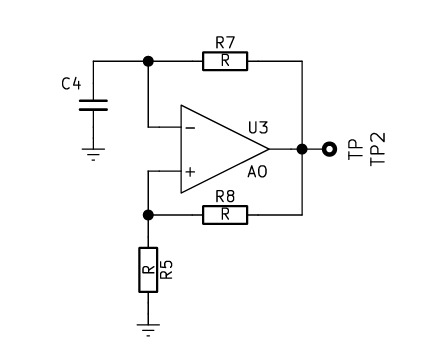
\includegraphics[width=0.5\textwidth]{multivibrador-astable.png}
    \caption{Multivibrador Astable con base en A.O}
    \label{fig:multivibrador-astable}
\end{figure}

\paragraph{Para el circuito de la figura \ref{fig:multivibrador-astable}, diseñar con el fin de obtener una oscilación de frecuencia 5.0kHz y amplitud 2V.\\}

Al usar un amplificador operacional UA741 alimentado con voltajes +VCC=10±1V y                     VEE= -10±1V este tendrá tensiones de saturación +Vsat = 8,005 V y –Vsat= -8,005 V, dichos valores fueron estudiados y comprobados en prácticas anteriores por lo cual serán utilizados como datos para esta práctica y para la práctica 3.3 del capítulo siguiente. 

\begin{equation}
    Vp = \frac{R_5}{R_5 + R_6} \cdot Vo_{\text{max}}
\end{equation}

Sustituyendo $Vp= 2V$ y $Vo = Vsat+$ se tiene

$$
2 = \frac{R_5}{R_5 + R_8}
$$

$$ R_8 = (6,005)R_5$$

si $R_5 = 3.3k $

entonces 

$$ R_8 = 10k$$


La frecuencia requerida es de 5,0kHz, despejando T de la ecuación (3) se obtiene el período.

$$ f = \frac{1}{T} $$


$$ T = \frac{1}{f} = 0.2ms$$

El periodo está dado por

\[
\mathcal{T} = t_1 + t_2 = - 2 R_\gamma \mathcal{C}_4 \ln \left( \frac{R_8}{2 R_5 + R_6} \right)
\]

Asumiendo que $C_4 = 10nF$ se tiene

\[
R_7 = - \frac{T}{2C_4 \ln \left( \frac{R_B}{2R_S + R_g} \right)} = \frac{0,2 \times 10^{-3}}{2 (100 \times 10^{-9}) \ln \left( \frac{1500}{2 \times 510 + 1500} \right)}
\]

$$R_7 = 22k\Omega$$


\begin{figure}[ht]
    \centering
    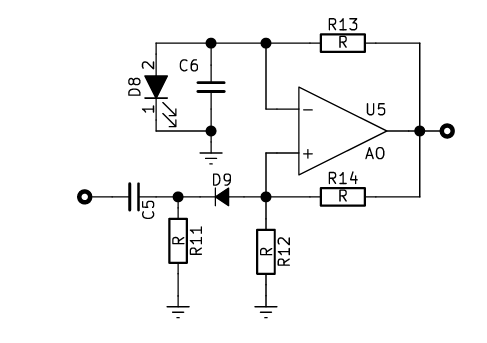
\includegraphics[width=0.5\textwidth]{multivibrador-monostable.png}
    \caption{Multivibrador Monostable con base en A.O}
    \label{fig:multivibrador-monostable}
\end{figure}


\paragraph{Para el circuito de la figura \ref{fig:multivibrador-monostable}, diseñar con el fin de obtener un tiempo de pulso de 10ms. }

El voltaje en la salida no inversora del amplificador (Vp), en el momento que ocurre el pulso negativo y D9 no conduce, está dado por la siguiente expresión: 

\[
V_{p3} = \frac{R_{12}}{R_{12} + R_{14}} Vo_{min}
\]

Suponiendo $R_{12} = 5.1k$ y $R_14 = 10k$

\[
V_{p3} = \frac{5.1k}{10k + 5.1k} (-8,005) = -6,38\,V
\]

$$V_p = 2.9$$

$R_{11}$ tiene que ser menor que $R_{12}$ por ejemplo $1k$

\[
R_{13} = \frac{t_c}{C_a \ln \left( \frac{V_{P3} - V_{SAT}}{V_{DB} - V_{SAT}} \right)} = \frac{10 \cdot 10^{-3}}{(100 \cdot 10^{-9}) \ln \left( \frac{-6,38 - (-8,005)}{1,5 - (-8,005)} \right)}
\]

$$R_{13} = 152k\Omega$$